% !TeX root = ../main.tex
\chapter{实机实验}
仿真实验与实机实验同步进行,也可以分成三个阶段:首先是搭建飞行平台,使得无人机可以在室外的GPS定位下进行遥控飞行,并且其动力足以应对后续的载荷增加;然后是在室内动作捕捉(motion capture)的外部定位下进行遥控飞行和轨迹跟踪,此时无人机上搭载机载电脑(companion computer)来提供动捕位姿信息和控制指令,控制算法仍然是PX4的四环pid控制;最后,在得到改成高阶全驱控制方法的飞控固件后,将其烧写进飞控板中,完成室内的遥控飞行和轨迹跟踪。
\section{飞行平台搭建}
一架用于室外GPS下飞行的无人机的基本组成部分有机架、螺旋桨、电机、电子调速器(简称电调)、飞控、GPS接收器、遥控接收机、与地面站通信的sik电台或wifi热点和电池。而动力套件指的是其中的螺旋桨、电机和电调,它们合在一起决定一架无人机的动力性能。
\begin{figure}[h]
  \centering
  \begin{minipage}[c]{0.33\textwidth}
    \centering
    \includegraphics[width=0.95\linewidth]{GPS飞机.jpg}
  \end{minipage} \hfill
  \begin{minipage}[c]{0.33\textwidth}
    \centering
    \includegraphics[width=0.95\linewidth]{GPS侧面.jpg}
  \end{minipage}\hfill
    \begin{minipage}[c]{0.33\textwidth}
      \centering
      \includegraphics[width=0.95\linewidth]{GPS底部.jpg}
  \end{minipage}
  \caption{用于室外飞行的四旋翼无人机多角度照片}
  \end{figure}


在所有的部件中,除了与地面站的通信装置的功能会被机载电脑替代,以及GPS接收器不再需要之外,其他的部件都不会有更改,因此只要在第一阶段的实验中将其调试定型,就可以继续在后续的实验中使用。在这一阶段,由于飞控、GPS接收器、sik电台和遥控接收机都已经有完善的产品,使用只需要正确的连线和配置,并且对后续的研究没有太大的影响,因此不是我们研究的重点。

而动力套则不然,它的性能需要和无人机的载重相匹配,并且会体现在后续的建模和控制之中。动力套内部的三者之间也存在很强的耦合关系,需要互相适配:电调的输入是飞控的电机控制信号,根据协议的不同可以分为模拟的pwm信号和数字的dshot、oneshot等,经过调制向电机输出三相交流电。三相交流电的频率决定无刷电机的转速上限,但由于外部载荷、空气阻力、机械摩擦等阻力矩以及反电动势等阻力因素的存在,三相交流电需要有足够高的电压才能克服这些阻力因素使电机转速达到设定值。这样的逻辑意味着,在设定的转速不变时,电调不需要改变三相交流电的频率而只用改变电压去克服外部不断波动的负载。在选型时要注意电调能提供的最大电流要超过电机的最大电流,并且留有$5\sim 10A$的余量。螺旋桨和电机的型号也需要互相匹配,使空气阻力的负载和电机的扭矩互相适应。电机的产品说明中会有详细的油门量与电压、电流、力效等输出的表格,要保证电机能提供的拉力足够带起载荷,并且出于抗扰和稳定的需要,要留出足够大的余量。如图\ref{电机表}所示,在$60 \%$的油门量时,单个电机就能提供$913.8g$的升力,而后续搭载了机载电脑的无人机质量仅有$873.1g$,推重比达到了4.18 。
\begin{figure}[!h]
  \centering
  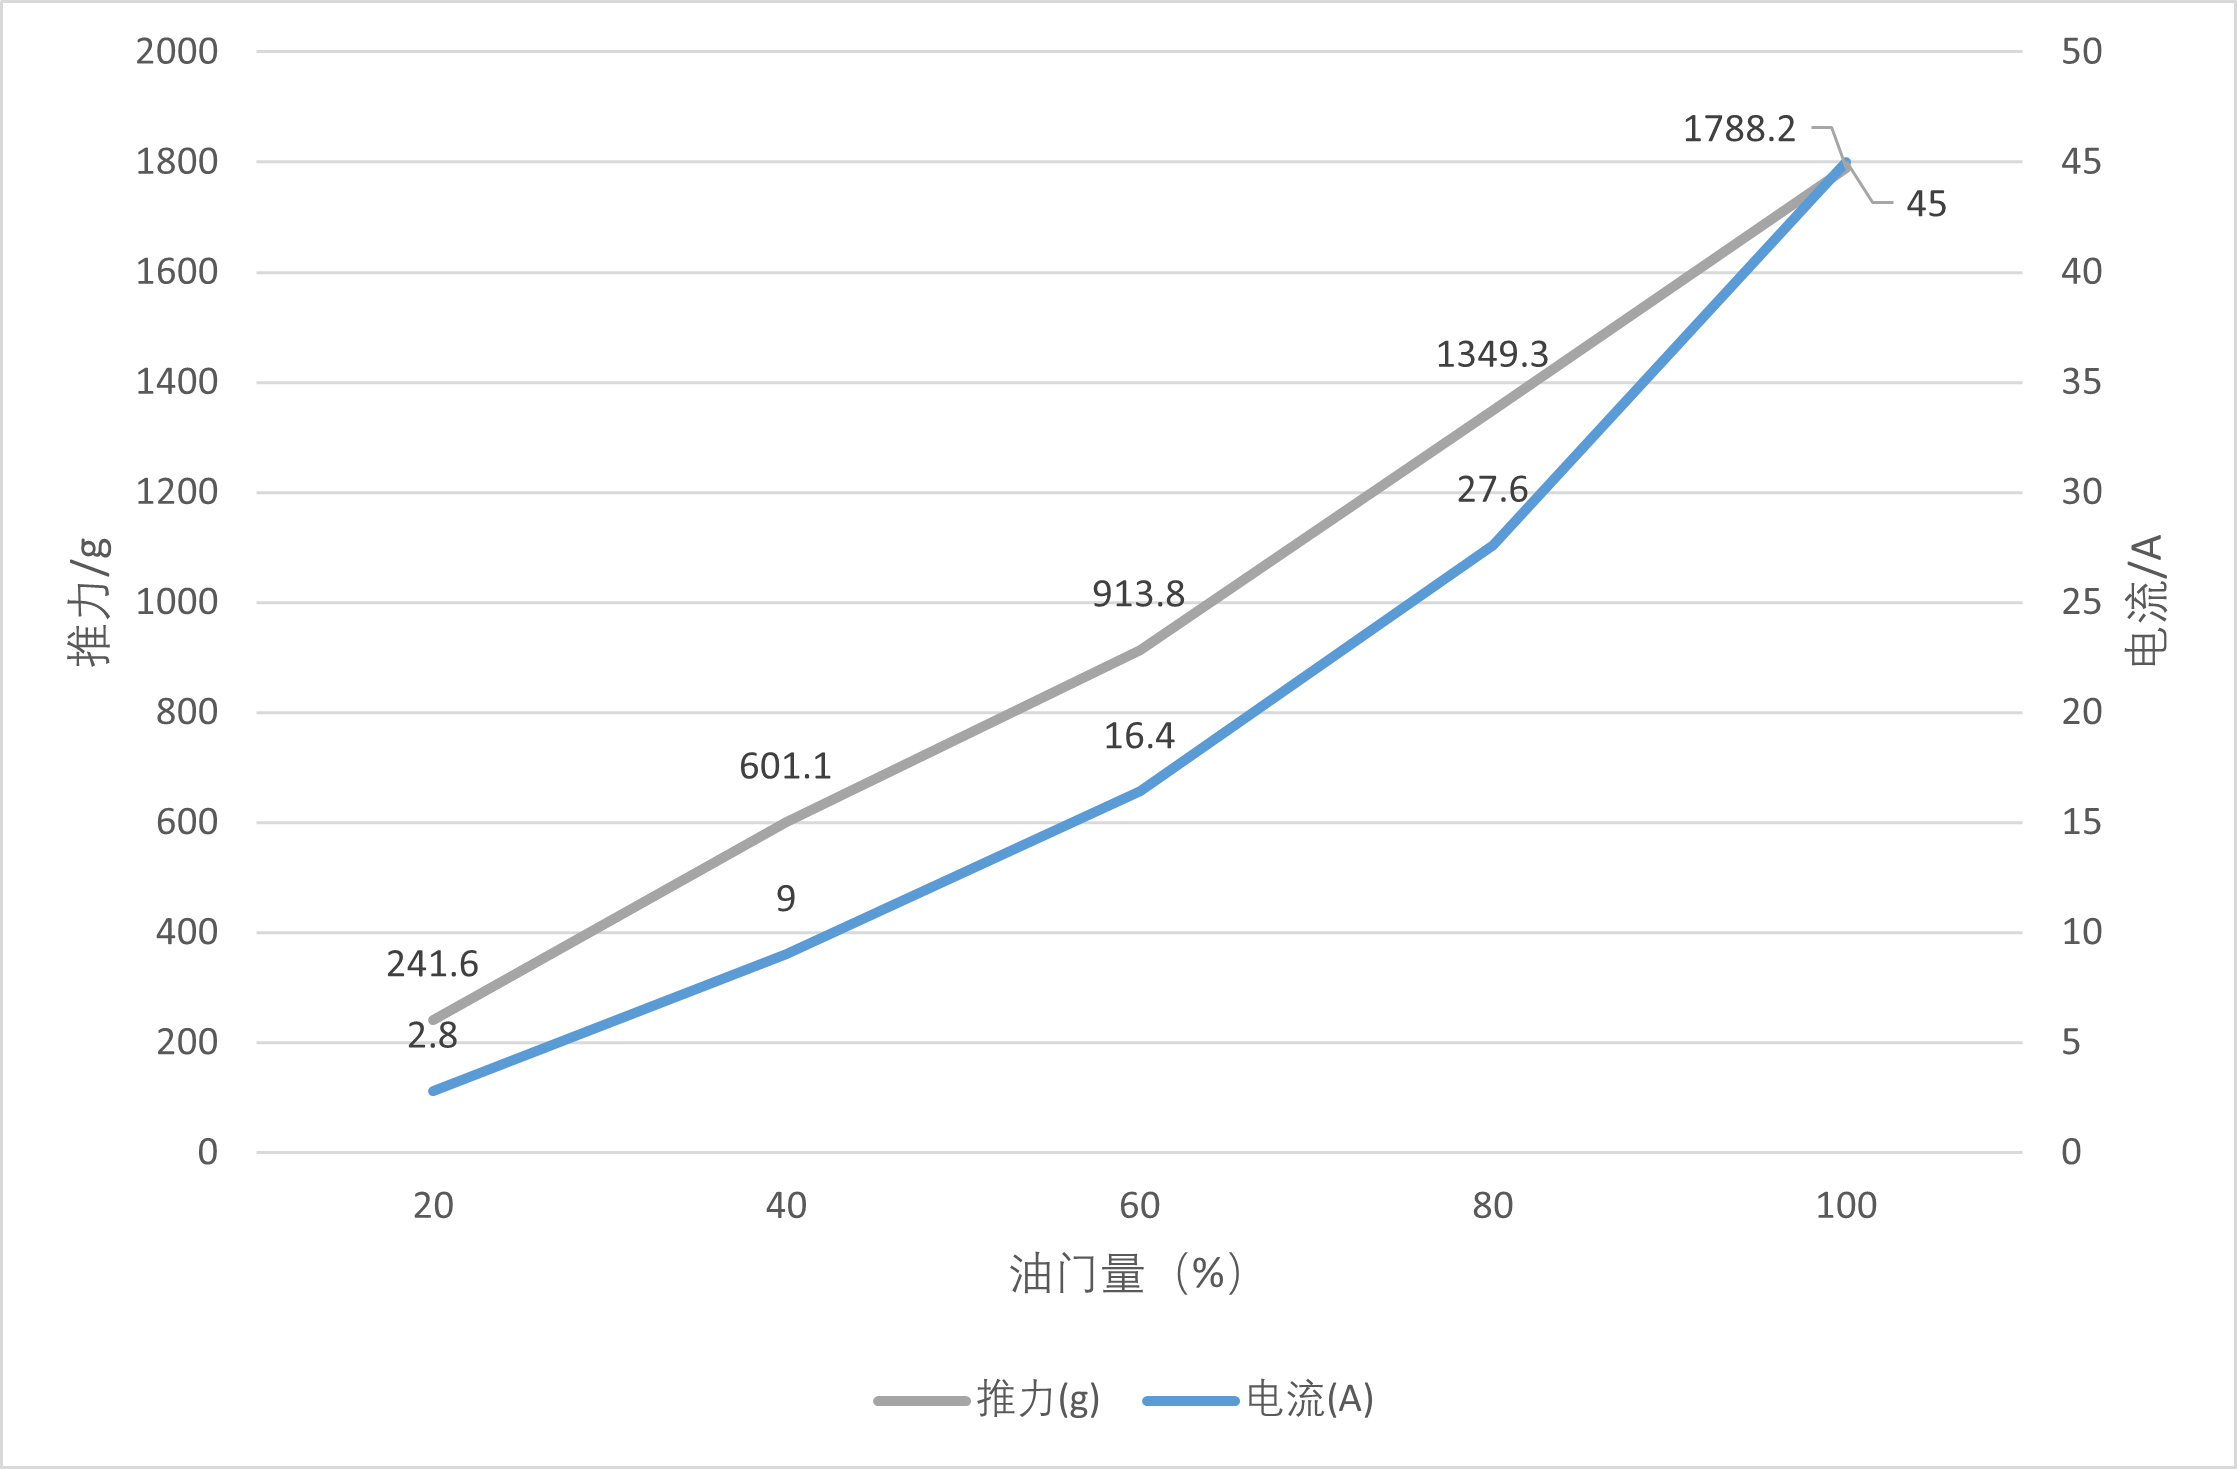
\includegraphics[width=0.7\textwidth]{电机表.png}
  \caption{Tmotor v2207 kv1950电机搭配51477-3螺旋桨 油门量与电流和推力关系图\cite{Tmotor2023}}
  \label{电机表}
\end{figure}

在几番摸索后,考虑到后续的机载电脑等载荷需要有足够的安装位置,我们选择了holybro品牌的QAV250机架作为平台,以及配套的PM06电源及电调模块,TMOTOR v2207 kv1950电机和pixhawk 6c mini飞控。在装配和接线后,在QGroundControl地面站中对飞控烧写PX4 v1.14版本的固件,并进行传感器校正和遥控器设置。最后,在卫星信号良好的室外进行了遥控器控制下的飞行实验。无人机能够很好地执行遥控器发布的飞行指令,悬停稳定,前进后退自如,飞行效果如图\ref{室外飞行}。

\begin{figure}[h]
  \centering
  \begin{minipage}[c]{0.33\textwidth}
    \centering
    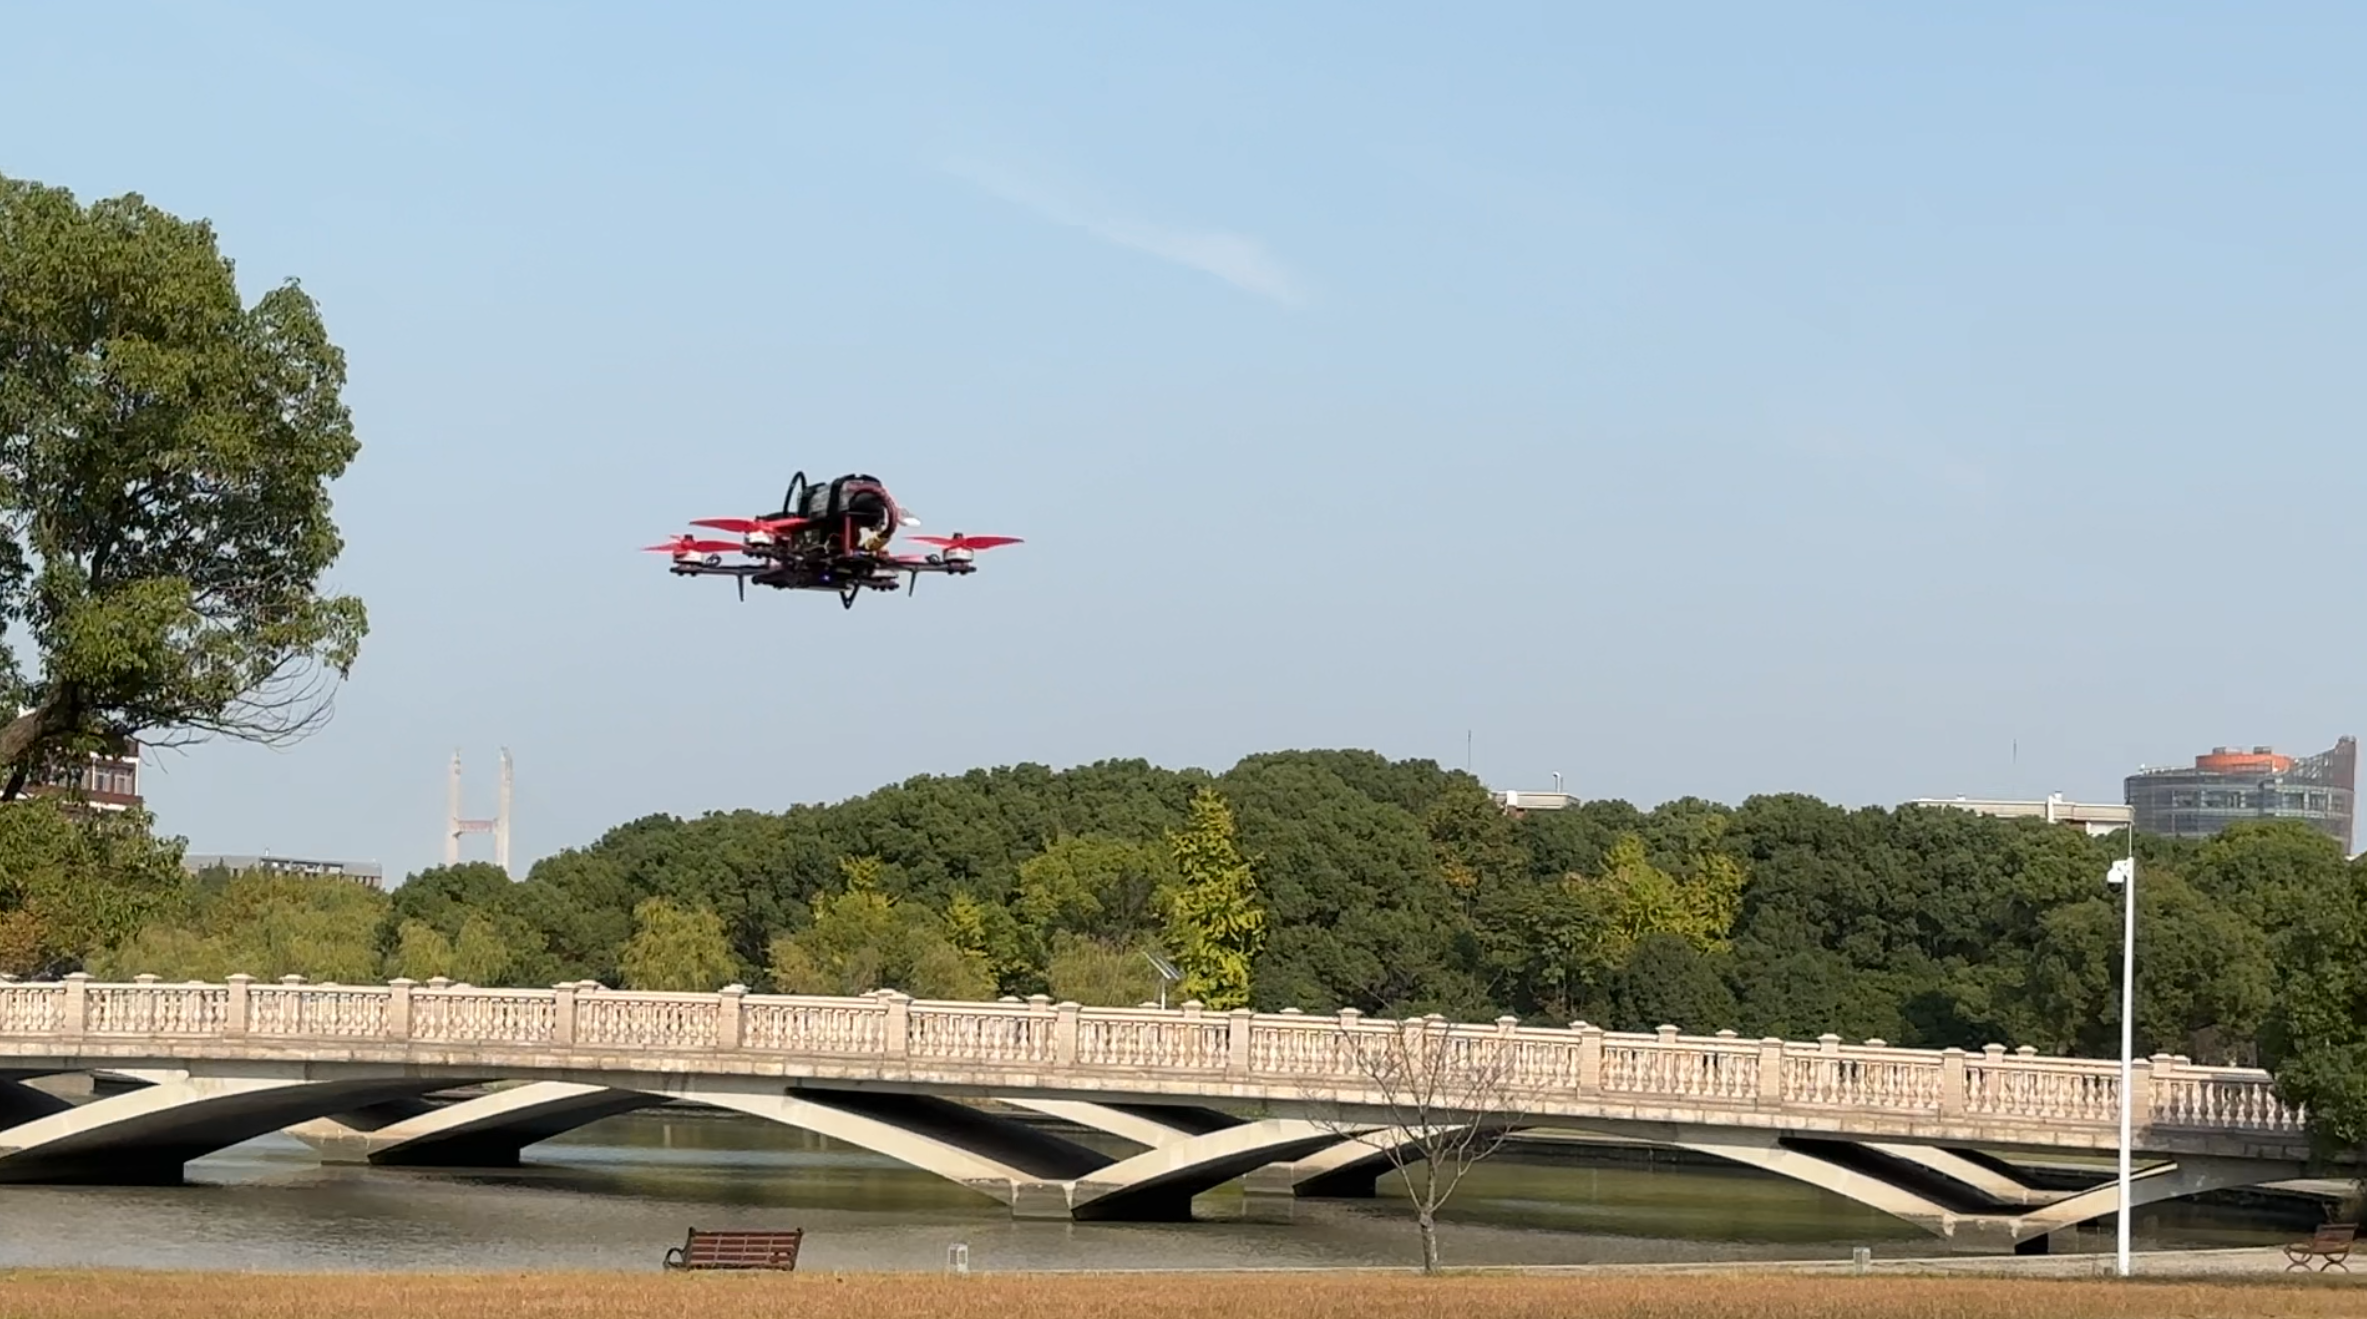
\includegraphics[width=0.95\linewidth]{室外飞行1.png}
  \end{minipage} \hfill
  \begin{minipage}[c]{0.33\textwidth}
    \centering
    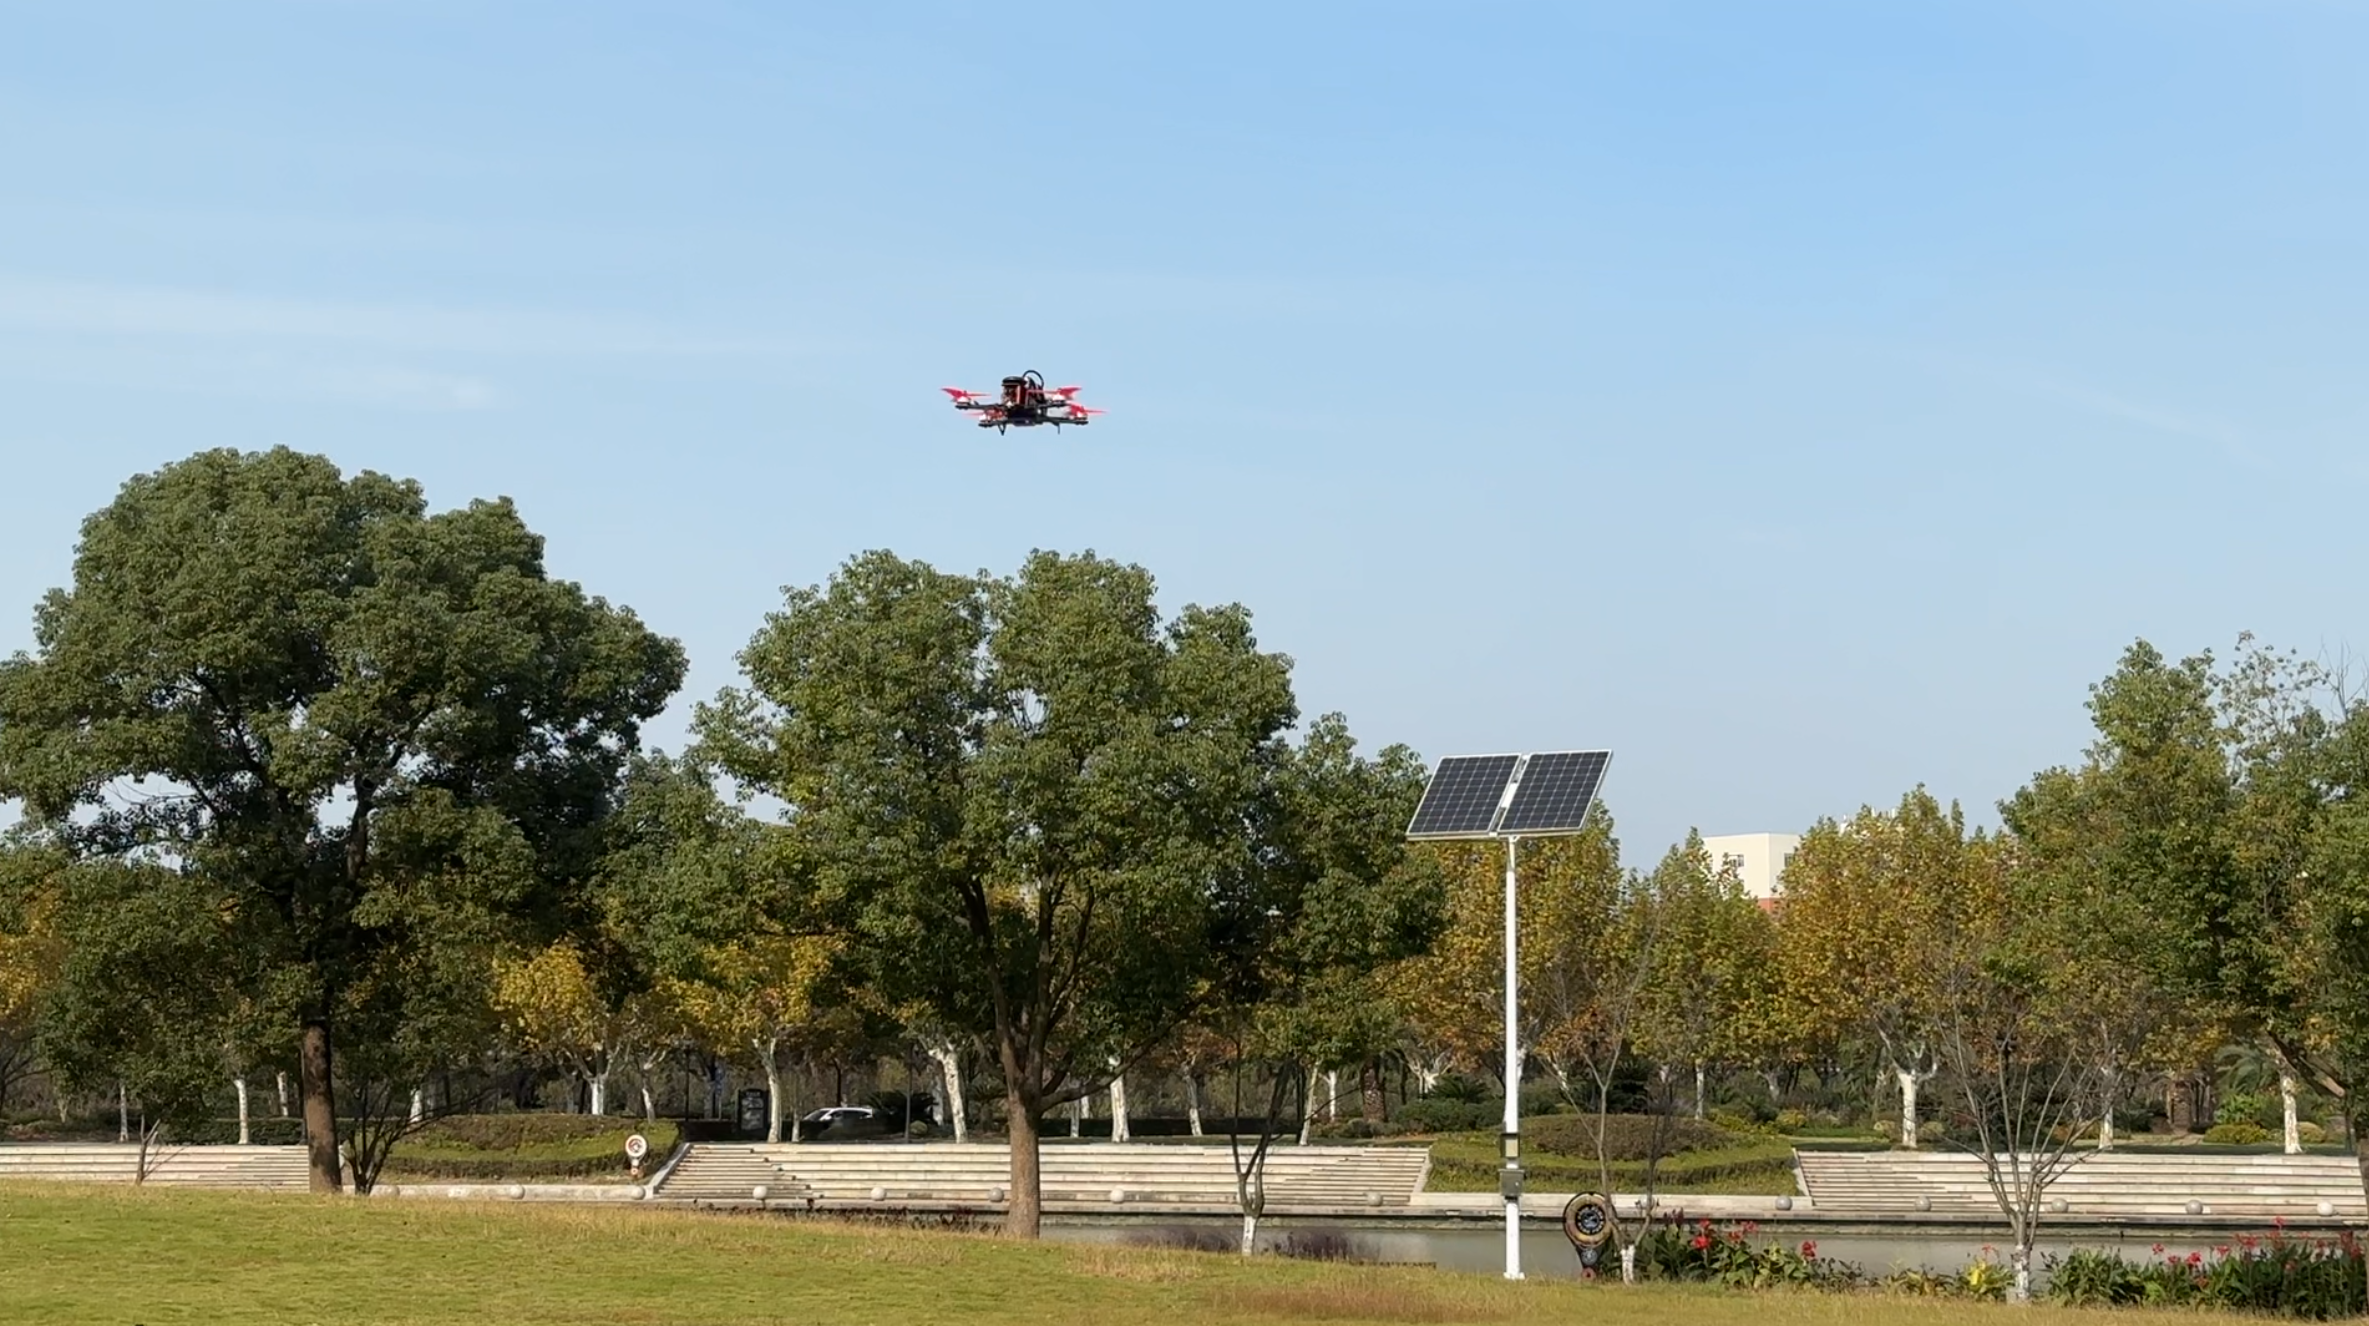
\includegraphics[width=0.95\linewidth]{室外飞行2.png}
  \end{minipage}\hfill
    \begin{minipage}[c]{0.33\textwidth}
      \centering
      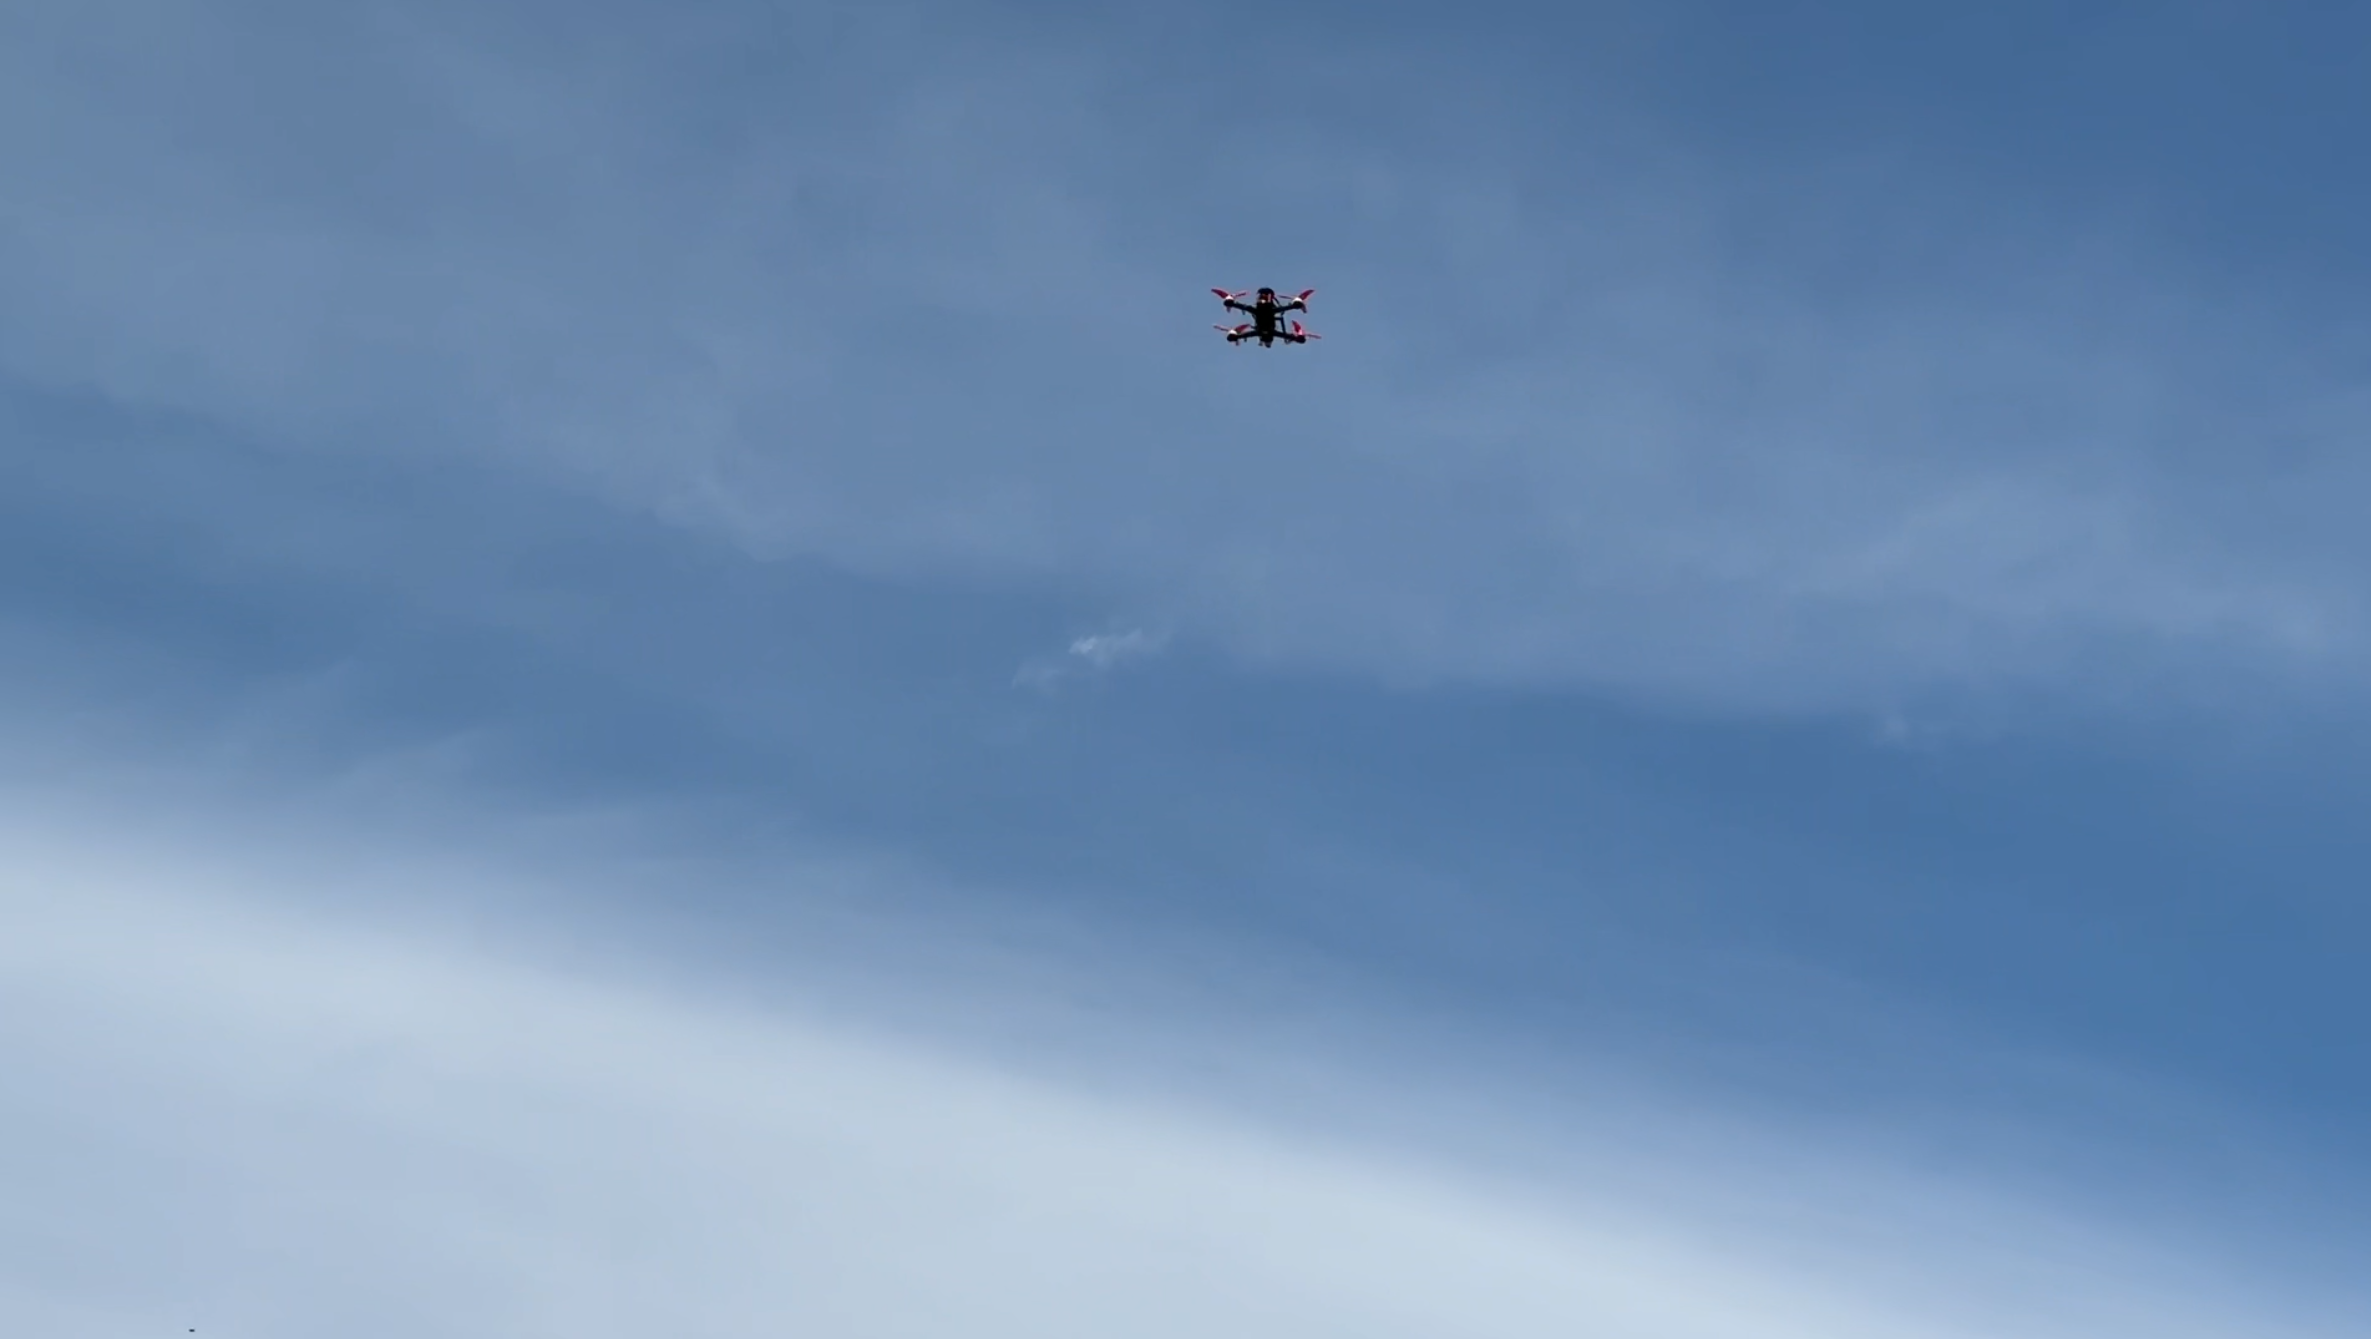
\includegraphics[width=0.95\linewidth]{室外飞行3.png}
  \end{minipage}
  \caption{位置模式下四旋翼室外飞行画面}
  \label{室外飞行}
  \end{figure}

  \section{搭载机载电脑的室内飞行}
室内飞行与室外飞行的主要区别在于位置信息的获得方式。由于室内没有GPS信号,位置信息的获取方式主要有动作捕捉、UWB、自主深度视觉定位和激光雷达等,其中动作捕捉的精度和稳定性最高,并且不用在飞机上增加额外的载荷,所以我们采用了动作捕捉作为本课题的定位方法。

我们采用8台动捕相机吊装在实验场地上方四周,实验场地的尺寸为$5m \times 4.6m \times 2.6m$。在当前配置下,可以达到亚毫米的定位精度和400hz的采样频率\cite{qingtong}。
\begin{figure}[!h]
  \centering
  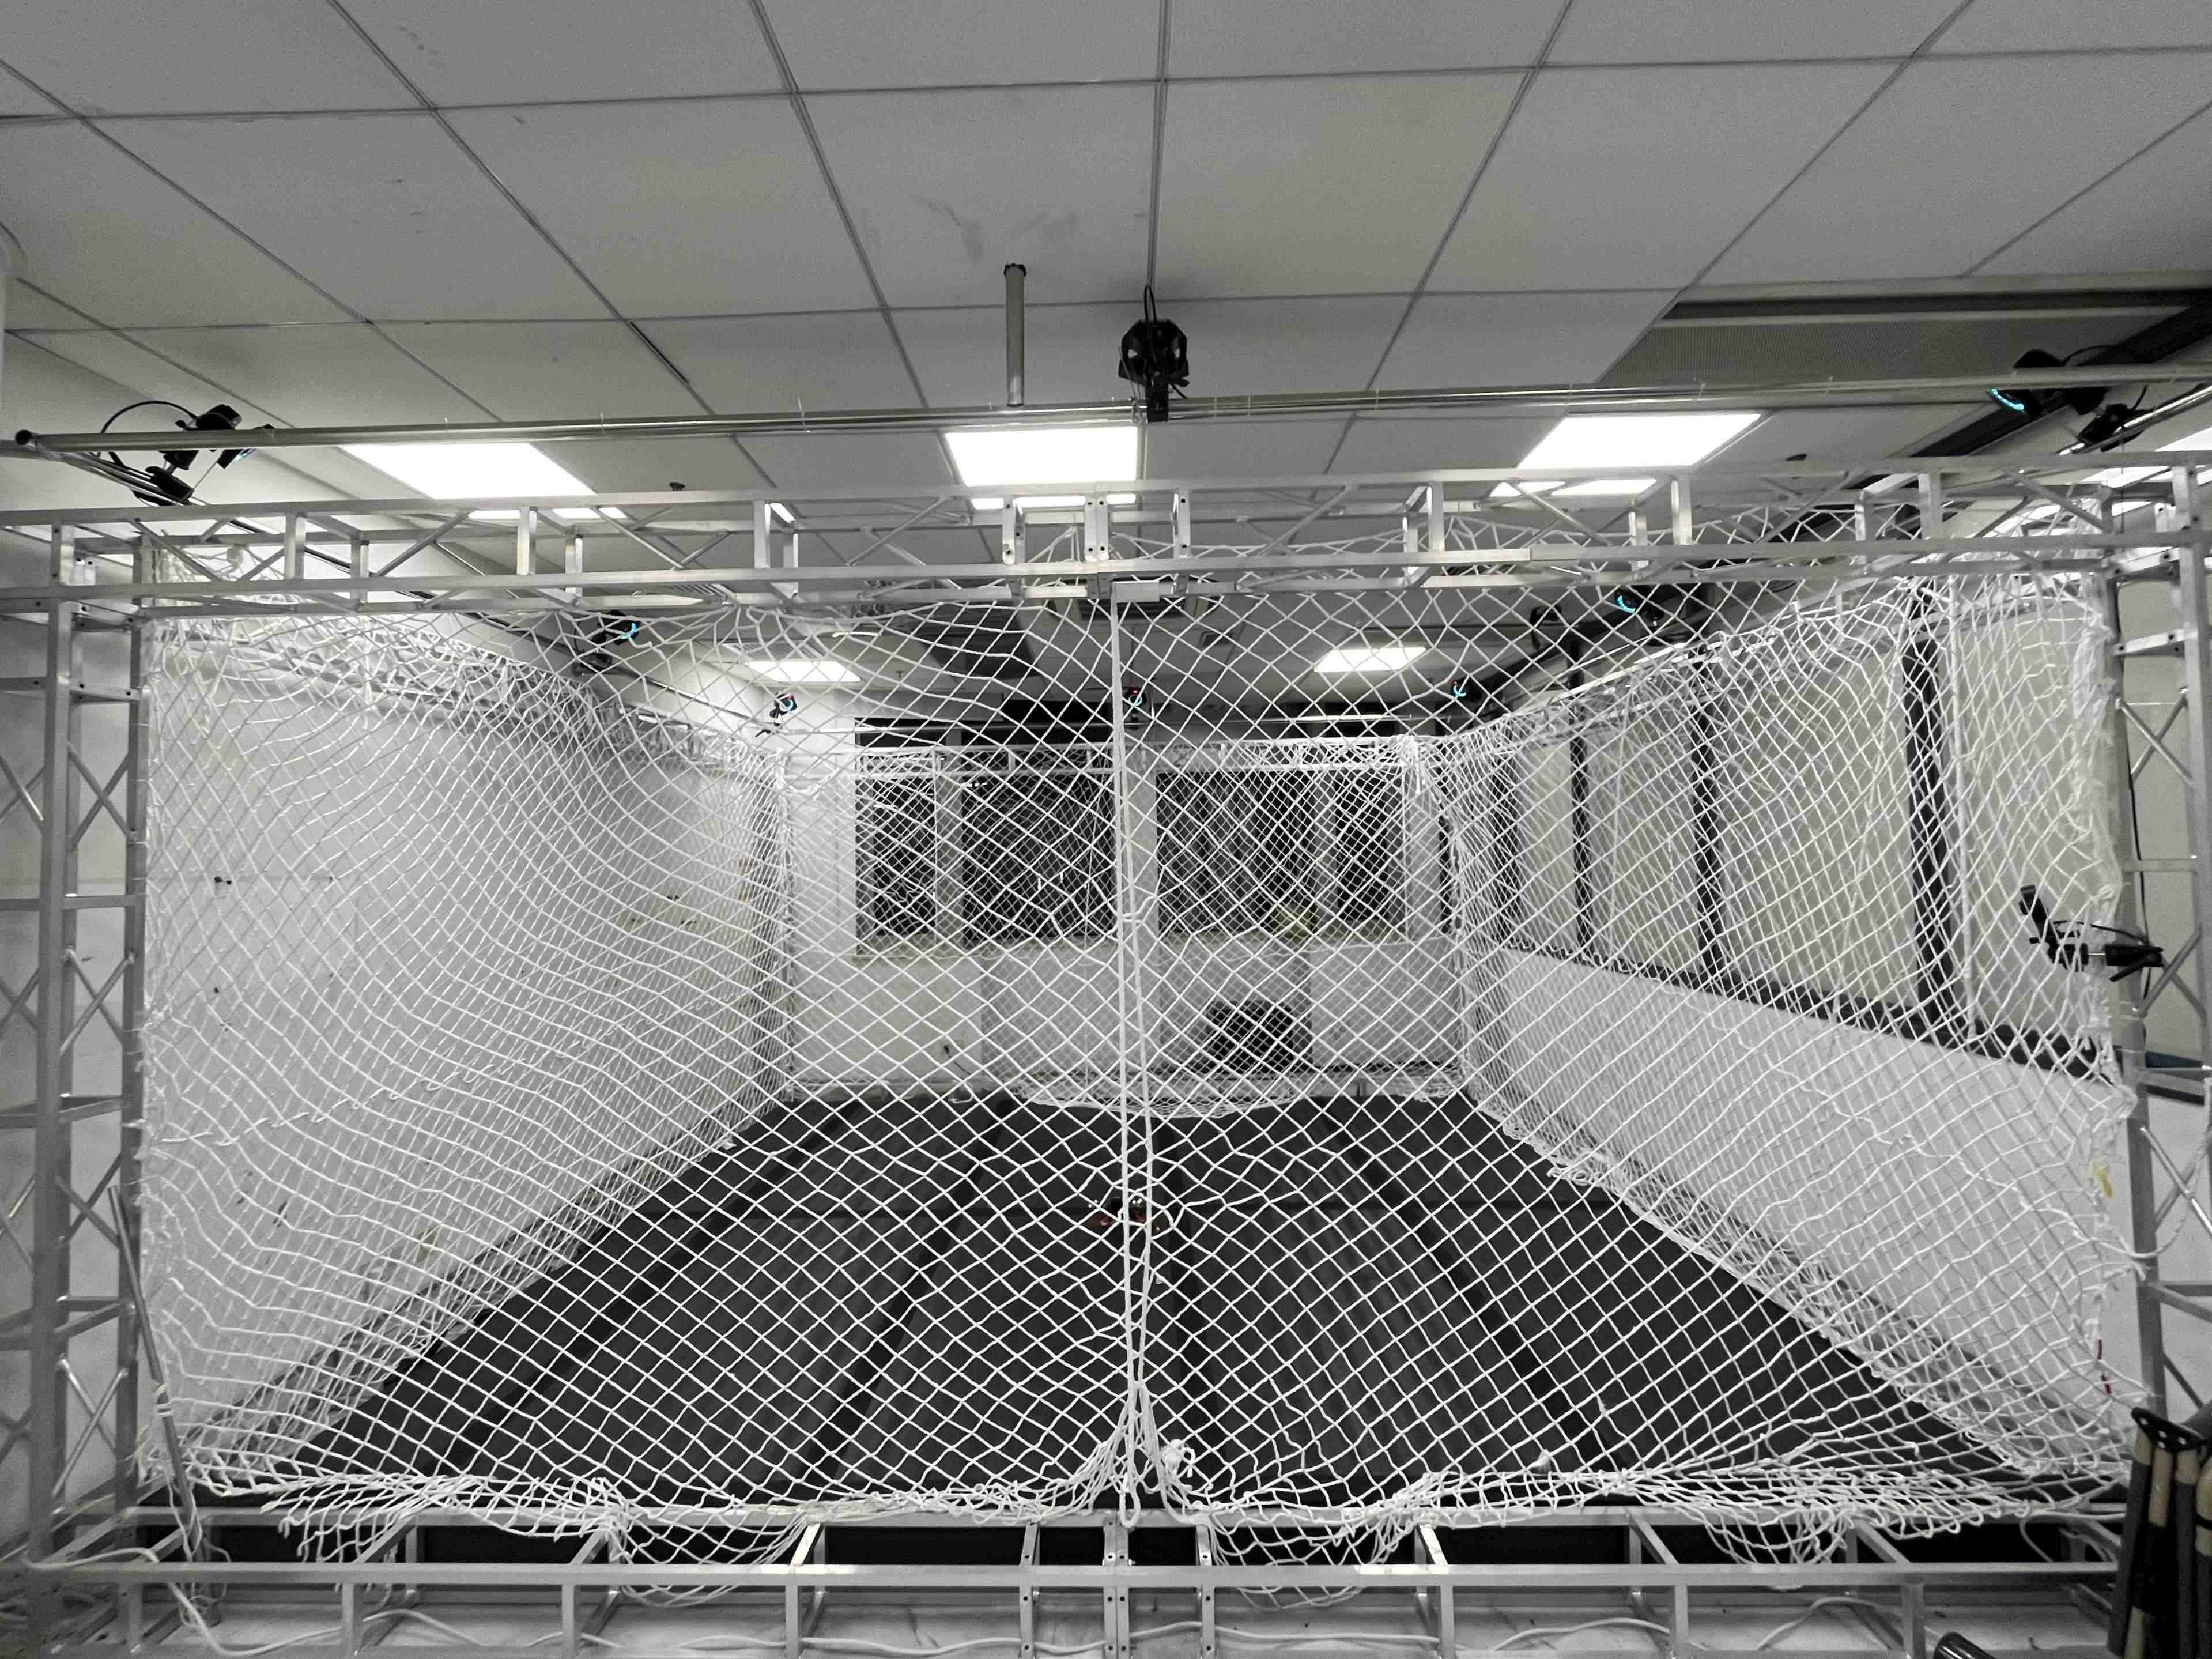
\includegraphics[width=0.6\textwidth]{动捕.jpg}
  \caption{动捕系统以及无人机防撞绳网}
  \label{动捕}
\end{figure}
动捕系统使用红外相机向目标发射红外光,使目标上固连的多个反光小球反射红外光,就能使相机捕捉到,效果如图\ref{反光小球}。

\begin{figure}[h]
  \centering
  \begin{minipage}[c]{0.48\textwidth}
    \centering
    \includegraphics[width=0.95\linewidth]{飞机反光球.jpg}
  \end{minipage}\hfill
    \begin{minipage}[c]{0.48\textwidth}
      \centering
      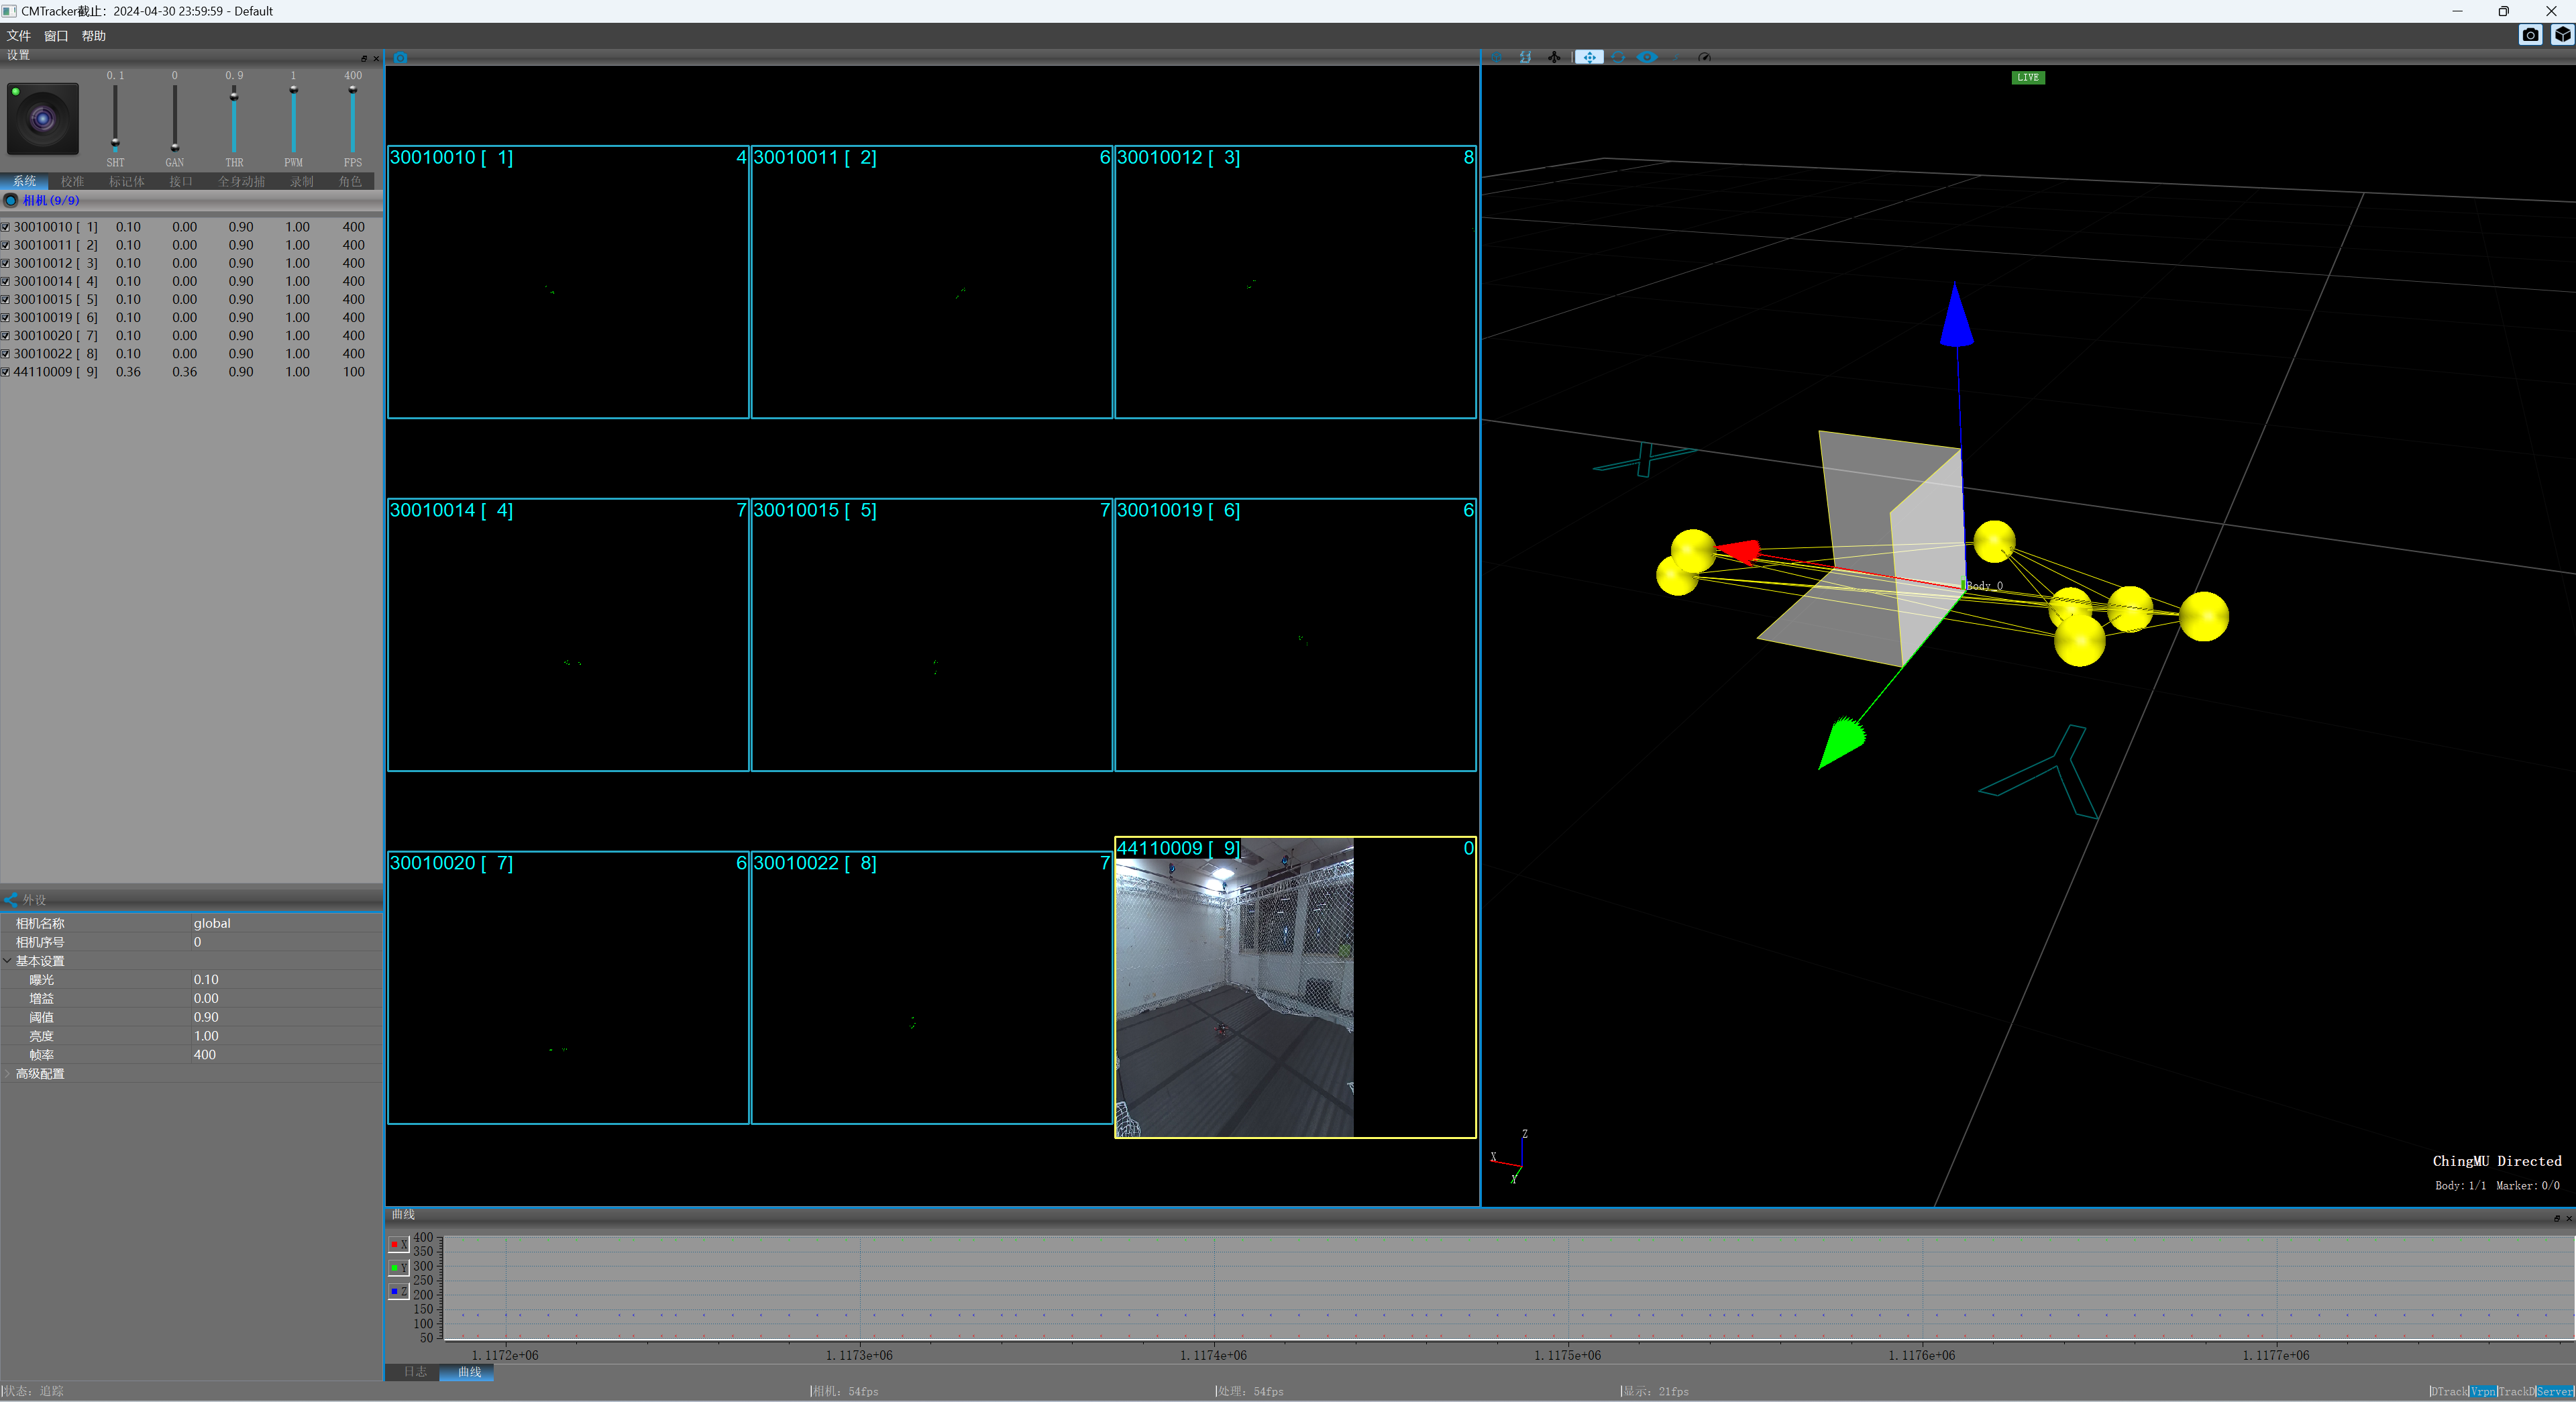
\includegraphics[width=0.95\linewidth]{动捕效果2.png}
  \end{minipage}
  \caption{动作捕捉定位反光小球}
  \label{反光小球}
  \end{figure}


由于相机通过扫场校准已知自身位置,多台相机的二维信息融合在一起就可以解算出目标的位置和姿态,如图\ref{动捕效果}。相机在拍到反光小球后首先在内部做一次图像处理,提取反光点位置,然后通过网线传到动捕服务器上。所有的相机和东部服务器都通过网线连在一台交换机上,形成一个局域网。动捕服务器在汇总了所有信息后解算出目标刚体的位置和姿态,然后以固定的数据报协议在其所在的所有局域网内广播。动捕服务器在用网线连接交换机之外,还和机载电脑连接同一个WIFI,也就是说动捕服务器同时处在两个局域网中,而机载电脑也可以通过WIFI这个局域网收到位姿广播。
\begin{figure}[!h]
  \centering
  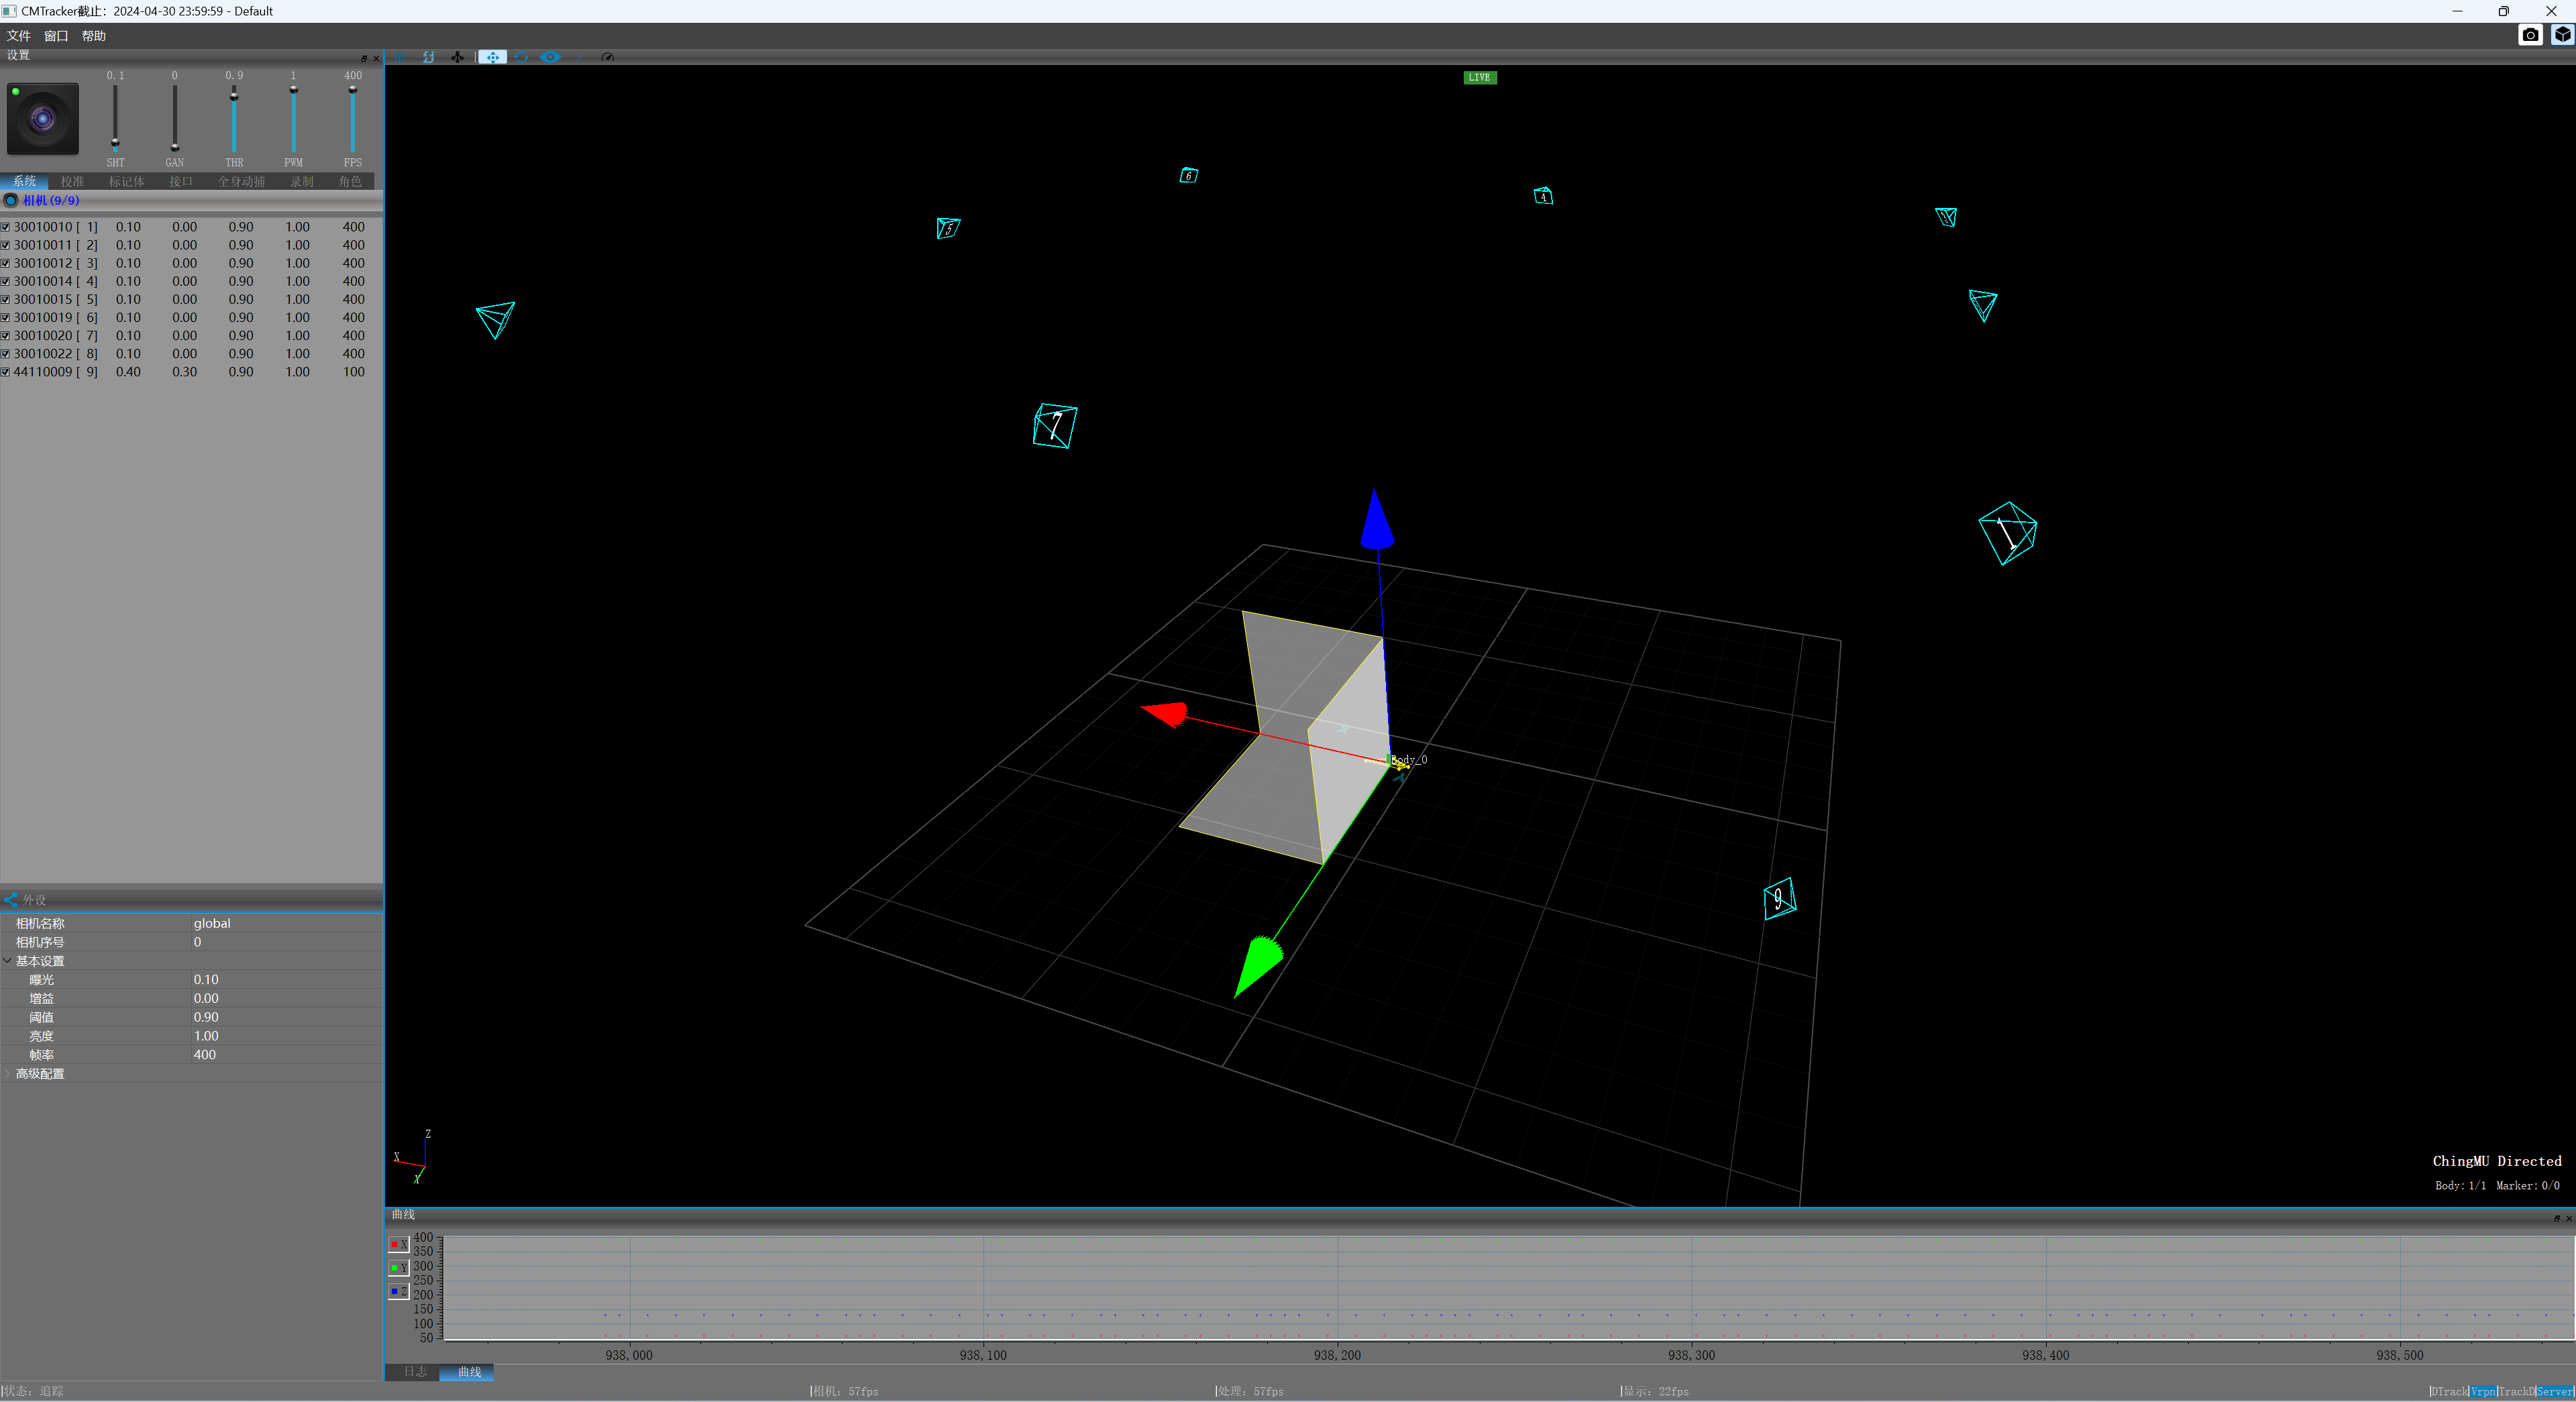
\includegraphics[width=0.6\textwidth]{动捕效果1.png}
  \caption{动捕效果}
  \label{动捕效果}
\end{figure}

在ros1的架构下,飞控和电脑需要存在有线连接才能通过运行mavros包下的px4.launch将飞控虚拟化为一个ros节点
